\artigotrue
\chapter{MODELO CONCEITUAL DE PEDOGÊNESE}
\shorttitle{Modelo Conceitual de Pedogênese}
\label{chap:chap03}
%\SweaveUTF8


\def\ptkeys{Província Geológica do Paraná. Bacia do DNOS. Rebordo do Planalto. Fatores de formação do solo. 
Pedogênese}

\begin{chapterabstract}{brazilian}{\ptkeys}
O presente documento apresenta o modelo conceitual de pedogênese -- descrição explícita dos fatores e 
processos de formação do solo que determinam as características do solo e o seu padrão de distribuição 
espaço-temporal -- da bacia de captação do reservatório do DNOS/CORSAN (Departamento Nacional de Obras de 
Saneamento/Companhia Riograndense de Saneamento), localizada no sul do Brasil. O clima é 
subtropical úmido sem estação seca definida. O relevo é plano a montanhoso (variação de altitude entre 139 e 
\SI{475}{\m}), com vales encaixados que influenciam a precipitação e o fluxo radiativo nas diferentes 
superfícies geomórficas. A geologia é constituída pela sequência de três formações geológicas: rochas 
sedimentares 
(arenito fluvial), seguidas de rochas ígneas (basaltos-andesitos toleíticos e vitrófilos, riólitos-riodacitos 
granofíricos) intercaladas por rochas sedimentares (arenito eólico). Depósitos do Quaternário aparecem nas 
partes mais baixas. A geomorfologia atual é resultado dos processos erosivos do Terciário e Quaternário. A 
dissecação atual é fraca devido ao clima que favorece a instalação e permanência de vegetação exuberante. Três 
unidades morfoestruturais são identificadas: no topo, o Planalto, com relevo suave-ondulado a ondulado, 
seguido pelo Rebordo do Planalto, com ampla variação altimétrica, declividade acentuada e escarpas abruptas; na 
base, a Depressão Periférica, com formas agradacionais de planície fluvial. Nas partes altas, a rede de 
drenagem apresenta padrão bem definido, geralmente retangular, determinada pelas falhas e/ou fraturas. Já nas 
áreas mais baixas, devido aos processos de deposição sedimentar e erosão fluvial, sua configuração é sinuosa. 
Ali 
encontram-se um lençol freático próximo da superfície do solo e cursos de água perenes. O uso da terra para 
produção agrossilvopastoril foi intenso em tempos pretéritos e resultou em forte degradação do solo. O 
abandono 
de muitas áreas degradadas permitiu a regeneração da vegetação natural, resultando na atual ocupação com 
florestas e vegetação secundária de \SI{\pm60}{\percent}. Em geral, o solo é pouco profundo devido ao 
predomínio de condições de forte declividade. É comum encontrar solo raso mesmo em áreas de maior estabilidade 
como fruto da degradação pelo uso agrícola. O solo é mais profundo no Planalto, nos terraços do Rebordo, nas 
coxilhas (colinas) de relevo suave-ondulado a ondulado, e nas planícies aluviais. A textura é mais fina e 
homogênea ao 
longo do perfil quando desenvolvido a partir de rochas vulcânicas. As características do solo nas planícies 
aluviais são determinadas pela presença constante de lençol freático próximo da superfície.
\end{chapterabstract}

% \def\enkeys{Paraná Geological Province, DNOS Catchment, Plateau Border, Soil formation factors, Pedogenesis}
%   
% \begin{chapterabstract}{english}{\enkeys}
% This document presents the conceptual model of pedogenesis -- an explicit description of soil-forming 
% factors and processes that determine the spatio-temporal distribution of soil properties  -- of the 
% catchment of the DNOS/CORSAN reservoir, located in southern Brazil. Climate is subtropical humid without a 
% dry season. Relief varies between plain and mountainous, with enclosed valleys (elevation ranging between 
% \num{139} and \SI{475}{\metre} above sea level) that determine rainfall volume and radiative flux on 
% different surfaces. The geology is composed of a sequence of three geological formations: consolidated 
% sedimentary rocks (fluvial sandstone), followed by basic and acid igneous rocks (andesite-basalt and 
% rhyolite-rhyodacite), interlayered with consolidated sedimentary rocks (aeolian sandstone). Unconsolidated 
% colluvial deposits of the Quaternary period occur in the lower portions of the landscape. Current 
% geomorphology is a result of erosive processes of the Tertiary and Quaternary. Landscape dissection is weak 
% due to the current climate that favours the installation and maintenance of an exuberant vegetation. There 
% are three morphostructural units: at the top, the \textit{Planalto} (Plateau), with gently-rolling to 
% sloping relief, followed by the \textit{Rebordo do Planalto} (Plateau Border), with wide altimetric 
% variation, steep slopes and abrupt cliffs; at the bottom, the \textit{Depressão Periférica} (Peripheral 
% Depression), composed of aggradational fluvial plains. In higher altitudes, the drainage network has a well 
% defined pattern, generally rectangular, determined by the faults and/or fractures. In the lower areas, its 
% configuration is sinuous due to sediment deposition and fluvial erosion, with the presence of water table 
% close to the surface and perennial water streams. Land use for agrosilvopastoral production was intense in 
% past times, resulting in severe soil degradation. Recent abandonment of many degraded areas allowed the 
% regeneration of natural vegetation, resulting in \SI{\pm60}{\percent} of the area being now occupied with 
% forest and secondary vegetation. The soil is predominantly shallow due to the dominance of steep slopes. 
% Even in gently-sloping terrain it is common to find shallow soils as a result of soil degradation, Deeper 
% soil can be found in the Planalto, in the terraces of the Rebordo, and in the small hills with 
% gently-rolling slopes and alluvial plains. Soil texture is finer and more homogeneous throughout the soil 
% profile in soil developed from igneous rocks. Soil features in the alluvial plains are determined by the 
% constant presence of the water table close to the surface.
% \end{chapterabstract}

\formatchapter

\section{APRESENTAÇÃO}
\label{sec:chap03-apresentacao}

\titlenote{Colaboraram na preparação deste documento: Pablo Miguel (UFPel), Jean Michel Moura Bueno (UFSM), 
Ricardo Simão Diniz Dalmolin (UFSM), Andrisa Balbinot (UFSM), Lúcia Helena Cunha dos Anjos (UFRRJ), Gustavo de 
Mattos Vasques (Embrapa Soils), e Gerard B. M. Heuvelink (ISRIC -- World Soil Information).}

A modelagem espacial do solo inicia com a definição de um \emph{modelo conceitual de pedogênese}. Um modelo 
conceitual de pedogênese constitui uma representação verbal da realidade sob estudo que inclui a descrição 
explícita dos fatores e processos de formação do solo que determinam as características do solo e o seu padrão 
de distribuição espaço-temporal. Isso requer a reunião de toda a informação ambiental disponível e aplicação 
dos conceitos de relação solo-paisagem, desenvolvimento do solo em catenas, ou outro modelo teórico de 
explicação da variação espacial do solo.

O presente documento apresenta o modelo conceitual de pedogênese da bacia de captação do reservatório do 
DNOS-CORSAN (Departamento Nacional de Obras de Saneamento-Companhia Riograndense de Saneamento), localizada na 
divisa entre os municípios de \itaara{} (ao norte) e \santamaria{} (ao sul), na porção sul da \baciaparana{}, 
estado do Rio Grande do Sul, Brasil (\autoref{fig:chap03-location}). A bacia de captação do reservatório do 
DNOS-CORSAN corresponde à cabeceira da bacia hidrográfica do \riovacacaimirim{}, tributário do \riojacui{} e, 
consequentemente, do \rioguaiba{} e da \lagoadospatos{}. A bacia de captação do reservatório do DNOS-CORSAN 
cobre uma área de \SI{\pm29}{\square\kilo\metre} e alimenta um reservatório com volume máximo de 
\SI{\pm3800000}{\cubic\metre} em uma área inundada de \SI{0,74}{\square\kilo\metre}. Este reservatório 
contribui com até \SI{30}{\percent} do abastecimento de água da cidade de Santa Maria \cite{Dias2003, 
DillEtAl2004, Miguel2010}.

\begin{figure}[!ht]
\centering
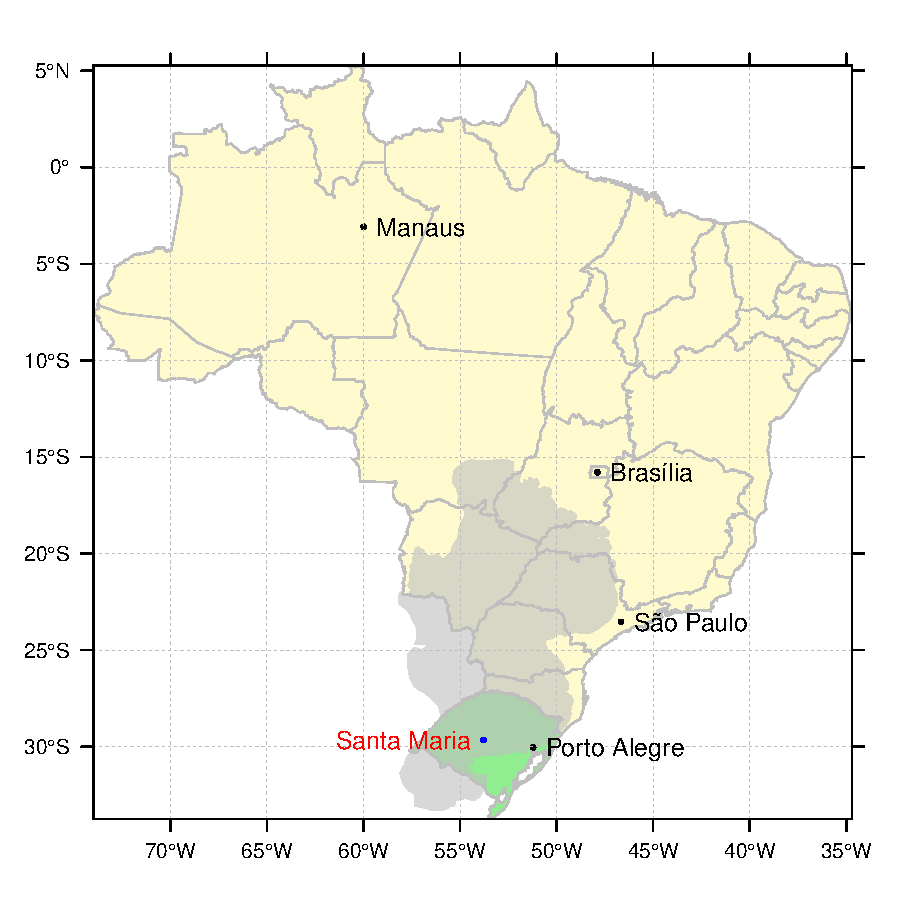
\includegraphics[width=0.90\textwidth]{fig/chap03-location}
\caption[Localização da bacia de captação do reservatório do DNOS-CORSAN, em Santa Maria, RS, 
Brasil]{Localização da bacia de captação do reservatório do DNOS-CORSAN no Município de Santa Maria, Estado do 
Rio Grande do Sul (em verde), Brasil, na porção sul da Província Geológica do Paraná (em cinza).}
\label{fig:chap03-location}
\end{figure}

\def\footsolosdors{\footnote{O grupo está registado no Diretório dos Grupos de Pesquisa no Brasil 
(\href{http://dgp.cnpq.br/dgp/espelhogrupo/9373361709890764}{DGP}) mantido pelo CNPq.}}

Os estudos em modelagem espacial do solo na bacia do DNOS -- abreviatura de bacia de captação do reservatório 
do DNOS-CORSAN -- iniciaram no ano de \num{2008} com o grupo de pesquisa \emph{Gênese, composição e 
comportamento dos solos do RS}\footsolosdors{}, sediado no Departamento de Solos da Universidade Federal de 
Santa Maria (\ufsm). Devido à limitação de recursos, o grupo de pesquisa optou por restringir seus estudos em 
modelagem espacial do solo à uma parte da bacia do DNOS. A área escolhida cobre \SI{\pm60}{\percent} de toda a 
bacia do DNOS, o que corresponde à uma área de \SI{\pm18}{\square\kilo\metre}. A área de estudo foi escolhida 
por apresentar acesso facilitado, além de englobar as todas as formações geológicas, geoformas, usos da terra, 
e vegetação presentes na bacia do DNOS (\autoref{fig:chap03-perspective}).

\begin{figure}[!ht]
\centering
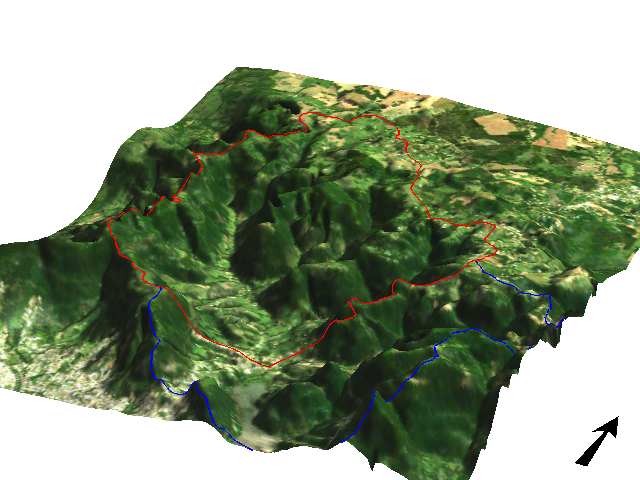
\includegraphics[width = 0.90\textwidth]{fig/chap03-perspective}
\caption[Localização da área de estudo na bacia do DNOS.]{Localização da área de estudo, em vermelho, na bacia 
de captação do reservatório do DNOS-CORSAN (em azul). A área de estudo, cujo relevo é bastante acidentado e o 
uso da terra predominante é floresta natural, corresponde a \SI{\pm60}{\percent} da bacia do DNOS.}
\label{fig:chap03-perspective}
\end{figure}

\section{CLIMA}
\label{sec:chap03-clima}

\def\footcfa{\footnote{Mais informações sobre o tipo climático Cfa podem ser encontrados na 
\href{https://pt.wikipedia.org/wiki/Clima_subtropical_\%C3\%BAmido}{Wikipedia}.}}

O clima local é classificado como Cfa\footcfa{} -- subtropical úmido sem estação seca definida --, com 
temperatura média anual de \SI{19,1}{\celsius}. As temperaturas podem alcançar \SI{>40}{\celsius}, no verão, e 
valores negativos no inverno \cite{HeldweinEtAl2009}. A precipitação média anual é de \SI{1708}{\milli\metre} 
bem distribuídos ao longo do ano \cite{Maluf2000}. Predominam os ventos do quadrante leste (frio, úmido e de 
intensidade fraca a moderada), oeste (frio, seco e de intensidade fraca a moderada) e norte (quente, seco e de 
intensidade moderada a forte) \cite{HeldweinEtAl2009}.

O padrão predominante das chuvas é o avançado, caracterizado por ter seu pico de maior intensidade no início 
da 
precipitação \cite{MehlEtAl2001}. As chuvas de maior intensidade ocorrem nos meses do final da primavera, 
verão e início do outono \cite{MouraBueno2012}. Como resultado desse padrão, as chuvas de inverno são as 
menos erosivas, mesmo que o conteúdo de água do solo permaneça elevado durante todo o período. O padrão de 
precipitação também é condicionado pelo relevo. Observações feitas em três locais durante o ano de \num{2011}, 
marcado por forte estiagem, mostram variação na lâmina total precipitada entre \num{1317} e \SI{1411}{\mm} 
\cite{MouraBueno2012}. Assim, o relevo plano a montanhoso, com vales encaixados, parece condicionar a formação 
de diferentes regiões microclimáticas, refletindo no volume e intensidade das chuvas \cite{MouraBueno2012}.

O relevo também deve condicionar o fluxo radiativo que atinge as diferentes superfícies. Apesar de não haver 
estudos que demonstrem a efetividade desse fenômeno na área, é reconhecido que grande parte da superfície em 
terrenos de topografia complexa é influenciada pelo efeito de sombreamento, sobretudo nas primeiras horas da 
manhã e no final da tarde \cite{OliphantEtAl2003}. Além disso, a declividade do terreno possui forte 
influência 
sobre o ângulo de interceptação da radiação solar pelas superfícies \cite{Birkeland1999}. Como consequência, 
deve ocorrer variações na temperatura e conteúdo de água no solo nas diferentes superfícies. Os meses de 
inverno são marcados por ainda menor disponibilidade de radiação solar devido à alta frequência de nevoeiros, 
sobretudo nas partes mais baixas, com valores normais de insolação de \SI{5,1}{\hour\per\day} 
\cite{HeldweinEtAl2009}. Além disso, devido à variação de altitude entre \num{139} e \SI{475}{\metre}, deve 
ocorrer diferença na temperatura da ordem de aproximadamente \SI{4}{\celsius} entre a parte mais baixa e a 
parte mais alta \cite{HeldweinEtAl2009}.

\section{GEOLOGIA}
\label{sec:chap03-geologia}

A geologia é bastante complexa, sendo constituída por três formações geológicas, além de depósitos coluviais 
e de aluvião do Quaternário. A literatura sobre o tema é vasta \cite{Bortoluzzi1974, Brasil1980, 
GasparettoEtAl1988, MacielFilho1990, Machado1998, PieriniEtAl2002, MarquesEtAl2005, Milani2005, Pinto2005, 
CPRM2007, Pedron2007, Sartori2009, NascimentoEtAl2010, WerlangEtAl2010, PedronEtAl2012}, e uma revisão da 
mesma é apresentada aqui.

% \begin{figure}[h]
%   \centering
%   \includegraphics[height=7cm]{figures/geo1988}
%   \caption{Mapa da geologia da AEPQ-SM publicado na escala 1:50.000 \citep{GasparettoEtAl1988}.\\Legenda: 
% SG-S - Sequência Superior da Formação Serra Geral, CT - Formação Caturrita, BT - Formação Botucatu, SG-I - 
% Sequência Inferior da Formação Serra Geral.}
%   \label{fig:geo1988}
% \end{figure}

\def\caturrita{\href{https://pt.wikipedia.org/wiki/Forma\%C3\%A7\%C3\%A3o_Caturrita}{Formação Caturrita}}

Na base da sequência estratigráfica, em elevações abaixo de \SI{\pm200}{\metre}, está a \caturrita{}, 
constituída por material sedimentar depositado em ambiente fluvial no Triássico Superior. Sua composição é 
diversa, apresentando seixos de siltito argiloso vermelho na base, seguido por arenito avermelhado de 
granulometria fina à média, composição quartzosa e matriz argilosa, podendo ainda conter considerável teor de 
feldspato, sobreposto por siltito e folhelho também avermelhados. Em geral, a granulometria do arenito é mais 
grosseira e menos argilosa na base da deposição. Devido à sua origem fluvial, a Formação Caturrita apresenta 
marcada estratificação cruzada acanalada e tabular. A origem fluvial também resulta em significativa variação 
espacial na granulometria do arenito, identificada pelo contraste entre áreas de maior cimentação e coesão, 
com 
outras de maior condutividade hidráulica. Imediatamente acima da Formação Caturrita encontra-se, ora a 
Formação Botucatu, ora a Sequência Inferior da Formação Serra Geral.

% \begin{figure}[h]
%   \centering
%   \includegraphics[height=7cm]{figures/geo1990}
%   \caption{Mapa da geologia da AEPQ-SM publicado na escala 1:25.000 \citep{MacielFilho1990}.\\Legenda: QD - 
% Depósitos do Quaternário, SG-S - Sequência Superior da Formação Serra Geral, CT - Formação Caturrita, BT - 
% Formação Botucatu, SG-I - Sequência Inferior da Formação Serra Geral.}
%   \label{fig:geo1990}
% \end{figure}

\def\serrageral{\href{http://pt.wikipedia.org/wiki/Forma\%C3\%A7\%C3\%A3o_Serra_Geral}{Formação Serra Geral}}

Em elevações entre \num{\pm200} e \SI{\pm350}{\metre} está a Sequência Inferior da \serrageral{} 
(basaltos-andesitos toleíticos). As rochas básicas são de coloração cinza-escura e são constituídas por 
plagioclásio cálcico, clinopiroxênio, magnetita e material intersticial de quartzo e material desvitrificado. 
Em elevações superiores a \SI{\pm350}{\metre} está a Sequência Superior da Formação Serra Geral (vitrófilos, 
riólitos-riodacitos granofíricos). As rochas ácidas apresentam cor cinza-clara, estrutura microcristalina e 
são constituídas por cristais e plagioclásio, clinopiroxênios, hornblenda uralítica e magnetita. A origem 
desse material remonta o Cretáceo, quando sucessivos derrames de lavas de origem vulcânica fissural ocorreram 
durante aproximadamente \num{10} milhões de anos em toda a Bacia do Paraná. Esses eventos ocorreram ao mesmo 
tempo em que iniciava-se a separação das plataformas continentais que hoje constituem a América do Sul e 
África, 
marcando o final da existência do supercontinente Pangeia.

\def\botucatu{\href{http://pt.wikipedia.org/wiki/Forma\%C3\%A7\%C3\%A3o_Botucatu}{Formação Botucatu}}

O arenito eólico constituinte da \botucatu{} é encontrado tanto assentado sobre a Formação Caturrita, como no 
interior da Formação Serra Geral (arenito \emph{intertrap}). Trata-se de um arenito quartzoso de granulometria 
fina à média, contendo feldspato alterado e cimentado por sílica ou por óxido de ferro, que lhe confere a 
coloração rosa-avermelhada. Sua deposição teve início no Cretáceo Inferior, período em que a Bacia do Paraná 
estava sob influência de clima desértico. Essa condição climática continuou durante todo o período em que 
ocorreram as dezenas de eventos de vulcanismo fissural, fazendo com que os mesmos fossem sucedidos por 
deposições eólicas de duração variável. Como a duração e a quantidade de material depositado pelos eventos de 
vulcanismo fissural era variável, assim como o intervalo de tempo entre cada novo evento e a intensidade das 
deposições de sedimentos eólicos, a espessura das camadas do arenito eólico e das rochas vulcânicas é bastante 
variável. Além disso, devido aos diversos eventos de subsidência que ocorreram no eixo central da Bacia do 
Paraná, com consequente soerguimento de suas bordas, as camadas dessas rochas possuem diferentes inclinações 
ao longo de sua faixa de exposição, sendo caracteristicamente ondulada e com suave tendência de inclinação 
para sudoeste.

As deposições do Quaternário são constituídas por depósitos coluviais e de aluvião. Em elevações entre 
\num{\pm200} e \SI{\pm300}{\metre} encontram-se depósitos coluviais de material proveniente de uma ou ambas as 
Formações Serra Geral (fragmentos de tamanho variado) e Botucatu. Em elevações abaixo de \SI{\pm200}{\metre} 
são mais comuns os depósitos coluviais de uma ou ambas as Formações Botucatu e Caturrita. Esses depósitos 
ocorrem de maneira descontínua nas encostas. Próximo aos cursos de água na porção mais baixa da bacia e no 
entorno do reservatório, encontram-se depósitos fluviais recentes, geralmente formados por fragmentos 
arredondados (seixos) de tamanho variável e/ou sedimentos arenosos. Em pequenas áreas abaciadas e mal 
drenadas, 
os sedimentos apresentam granulometria mais fina.

\section{GEOMORFOLOGIA}
\label{sec:chap03-geomorfologia}

A área de estudo está situada na porção sul da Bacia Sedimentar do Paraná. Assim, as geoformas atuais são 
resultado dos processos erosivos que ocorreram durante o Terciário e o Quaternário \cite{Sartori2009}, após as 
últimas deposições de lavas vulcânicas e de sedimentos eólicos. Durante esse período, a esculturação da 
paisagem foi determinada pelas alternações entre climas úmidos, semiáridos e áridos \cite{Sartori2009}. 
Atualmente, o clima subtropical úmido favorece a instalação e permanência de uma vegetação mais eficiente na 
redução do processo de dissecação da paisagem \cite{Sartori2009, NascimentoEtAl2010}. Isso permite que as 
superfícies geomórficas atinjam maior estabilidade e maturidade, embora o uso agrícola das terras tenha 
acelerado os processos erosivos na área.

% \begin{figure}[h]
%   \centering
%   \includegraphics[height=7cm]{figures/dem90}
%   \caption{Modelo digital de elevação da AEPQ-SM com resolução espacial de 90~m (SRTM DEM versão 4) 
% \citep{JarvisEtAl2008}.}
%   \label{fig:dem90}
% \end{figure}

As unidades morfoestruturais que abrangem a área são o Planalto e o Rebordo do Planalto da Bacia do Paraná 
\cite{NascimentoEtAl2010}. O Planalto é marcado por relevo suave-ondulado a ondulado, com formas denudacionais 
de superfícies planas com topos convexos (fluxo hídrico divergente). Nesses locais, as vertentes assumem a 
forma convexa levemente ondulada \cite{NascimentoEtAl2010}, muitas vezes encaixadas em falhas e/ou fraturas. 
Já o Rebordo do Planalto é caracterizado pela ampla variação altimétrica, declividade acentuada e escarpas 
abruptas, apresentando formas denudacionais com topos convexos (fluxo hídrico divergente), aguçados e em 
formas de escarpas. Nesses locais, as vertentes assumem forma retilínea com grande desnível 
\cite{NascimentoEtAl2010}, muitas vezes interrompidas por degraus ou patamares, na maioria das vezes 
encaixadas 
em falhas e/ou fraturas. Esses patamares são resultado da ação diferencial dos processos denudacionais sobre a 
paisagem, geralmente condicionados pela resistência do material de origem, seja ela química/mineralógica 
(rochas vulcânicas básicas vs. ácidas), física/granulométrica (rochas vulcânicas versus sedimentares), ou 
estrutural (padrão de diaclasamento vertical vs. horizontal das rochas vulcânicas) \cite{Holtz2003, 
Pedron2007, 
StreckEtAl2008}. Entretanto, em algumas situações, os patamares são formados por depósitos coluviais -- mesmo 
nas partes altas do Rebordo do Planalto -- resultantes de movimentos de massa causados por eventos 
pluviométricos de elevada intensidade e/ou duração \cite{PinheiroEtAl2004, PaisaniEtAl2010}. Nesses casos, os 
patamares possuem menor dimensão e maior declividade. Em outras situações, os patamares coluviais, sobretudo 
aqueles originados dos arenitos da Formação Botucatu, formam 
vertentes alongadas e com menor inclinação, que chegam até a margem dos cursos de água.

% \begin{figure}[h]
%   \centering
%   \includegraphics[height=7cm]{figures/dem10}
%   \caption{Modelo digital de elevação da AEPQ-SM com interpolado de curvas de nível com 10~m de 
% equidistância 
% \citep{DSG1980, DSG1992, DSG1992a}.}
%   \label{fig:dem10}
% \end{figure}

Apesar da área de estudo ser abrangida pelas unidades morfoestruturais do Planalto e do Rebordo do Planalto
da Bacia do Paraná, as características geomorfológicas das porções mais baixas da paisagem são similares 
àquelas encontradas na Depressão Periférica. Essas áreas são marcadas pelo acúmulo de sedimentos provenientes 
do Planalto e do Rebordo, formando planícies aluviais que se intercalam entre as coxilhas (denominação 
regional de colinas). Essas áreas são caracterizadas pela presença de formas agradacionais de planície fluvial 
e formas denudacionais de topos convexos e de superfícies planas. As últimas correspondem às coxilhas de 
algumas dezenas de metros de altitude, geralmente formadas sobre o substrato da Formação Caturrita 
\cite{GasparettoEtAl1988}, e assentadas na base do Rebordo do Planalto. Essas coxilhas constituem 
divisores de água de pequena amplitude que auxiliam na subdivisão da área em pequenas sub-bacias 
\cite{Marins2004, Sartori2009}. Nesses locais as vertentes costumam ser alongadas e assumem a forma 
predominantemente côncava devido aos processos de deposição sedimentar e erosão fluvial, apesar dos mesmos 
serem muito fracos sob a atual condição climática 
\cite{NascimentoEtAl2010, WerlangEtAl2010}.

A grande heterogeneidade geomorfológica da área de estudo se traduz em uma grande heterogeneidade textural 
do relevo, ou rugosidade, resultante da ação climática ao longo do tempo geológico \cite{NascimentoEtAl2010}. 
Entretanto, em menor escala, a ação antrópica também atua sobre a configuração geomorfológica da área. O 
principal efeito se deu pela erosão da camada superficial do solo, cultivado intensivamente sem o uso de 
práticas conservacionistas ao longo de inúmeras décadas \cite{Menezes2008, Sturmer2008, Miguel2010, 
SamuelRosaEtAl2011a}. Além disso, a abertura de caminhos para acesso às áreas de produção nos patamares do 
Rebordo do Planalto e nos topos de morros proporcionou a formação de canais de concentração e escoamento dos 
fluxos hídricos, levando à formação inicial de voçorocas. Obras de maior expressividade, como ferrovias, ruas 
e rodovias pavimentadas, conjuntos habitacionais e construções isoladas, as quais envolvem operações de 
terraplanagem e aterramento, também resultaram em modificações localizadas na geomorfologia da área. Por fim, 
a construção do reservatório possibilitou a formação de uma área de agradação da paisagem bastante estável em 
seu entorno, uma vez que o sedimento removido do Planalto e do Rebordo do Planalto não são mais transportados 
a jusante.

\section{HIDROGRAFIA}
\label{sec:chap03-hidrografia}

A hidrografia da área é condicionada pelas condições geomorfológicas, geológicas, pedológicas e climáticas, ao 
mesmo tempo em que exerce forte influência sobre a modelagem da paisagem \cite{NascimentoEtAl2010}. Como a área 
é 
abrangida pelas unidades morfoestruturais do Planalto e do Rebordo do Planalto da Bacia do Paraná, a drenagem 
apresenta um padrão bem definido, geralmente retangular, determinado pelas falhas e/ou fraturas 
\cite{Bortoluzzi1974, GasparettoEtAl1988, NascimentoEtAl2010}. A própria formação da bacia do DNOS se deve 
a existência de falhas e/ou fraturas \cite{GasparettoEtAl1988}. A principal e maior delas localiza-se no eixo 
central da bacia, onde atualmente está localizado o leito do rio Vacacaí-Mirim. Quanto aos tributários do rio 
Vacacaí-Mirim, a maioria possui o leito assentado sobre outras falhas e/ou fraturas de menor dimensão 
perpendiculares àquela do eixo central da bacia.

Nas áreas mais baixas, cujas características geomorfológicas se assemelham à Depressão Periférica, a drenagem 
apresenta configuração serpenteada, resultado dos processos de deposição sedimentar e erosão fluvial 
\cite{PaivaEtAl2001, SutiliEtAl2009}. Como o relevo é plano a suave-ondulado, e as vertentes longas e 
predominantemente côncavas, o lençol freático fica próximo da superfície do solo. A variação das condições 
meteorológicas ao longo do ano fazem com que o lençol freático apresente flutuação significativa, mantendo o 
conteúdo de água do solo elevado durante os meses mais frios (menor evapotranspiração) \cite{HeldweinEtAl2009}.
Isso também favorece a ocorrência de inundações, sobretudo nas proximidades dos cursos de água e do 
reservatório \cite{Goldani2006}.

Muitos cursos de água localizados no Planalto, no Rebordo do Planalto e nas coxilhas assentadas em sua base, 
são sazonais. Em geral, esses cursos de água estão em atividade apenas nos meses mais frios do ano, quando a 
disponibilidade de água no ambiente é maior, ou durante os eventos de precipitação de forte intensidade, que 
ocorrem nos meses de verão \cite{HeldweinEtAl2009, MouraBueno2012}. Os cursos de água do Rebordo do Planalto 
costumam apresentar leito raso e pedregoso, muitas vezes assentado sobre rochas da Formação Serra Geral 
\cite{SutiliEtAl2009}. Já os cursos de água localizados nos patamares e coxilhas costumam ser rasos, se 
assentados sobre as rochas da Formação Caturrita, ou profundos, se assentados sobre as rochas da Formação 
Botucatu ou depósitos coluvionares, formando voçorocas. Segundo relatos de alguns dos moradores mais antigos, 
muitas nascentes e pequenos cursos de água já perderam totalmente sua atividade, sobretudo quando localizadas 
no interior ou à jusante de áreas de uso antrópico.

Dado que a declividade e o desnível entre a parte mais baixa e a parte mais alta da área são acentuados, as 
cheias costumam apresentar velocidade e vazão bastante grandes \cite{PaivaEtAl2001, SutiliEtAl2009}. Em média, 
nos \SI{7}{\km} de extensão do rio Vacacaí-Mirim, da nascente até o reservatório, a declividade média é de 
\SI{0,03}{\m\per\m}. Isso representa um desnível de \SI{\pm210}{\m}, o que resulta em um tempo de concentração 
da bacia estimado em \SI{3}{\hour} \cite{PaivaEtAl2001}. Essas características causam erosão severa nas 
margens dos cursos de água nas áreas mais baixas (depósitos aluviais), sobretudo nos raios externos das 
curvas, onde a velocidade da água é maior \cite{SutiliEtAl2009}. Em alguns trechos, os cursos de água chegam a 
ter sua largura duplicada em menos de uma década, resultando no aumento da sinuosidade e do nível de fundo 
\cite{PaivaEtAl2001}. Esses eventos comprometem áreas de produção, bem como a estrutura de residências e vias 
públicas localizadas nas margens dos cursos de água. Grande parte do material removido das margens dos cursos 
de água é transportado para dentro do reservatório, que já perdeu mais de \SI{30}{\percent} de sua capacidade 
inicial de armazenamento de água \cite{DillEtAl2004}.

\section{USO DA TERRA}
\label{sec:chap03-landuse}

A área de estudo já foi intensamente ocupada em tempos pretéritos. Isso é evidenciado pela grande quantidade, 
extensão e boa distribuição da rede viária em toda a sua área. Além disso, a área é cortada por uma estrada 
férrea e avizinha uma rodovia federal, ambas muito movimentadas. Entretanto, nas últimas décadas, muitos 
caminhos internos das propriedades rurais foram desativados, fruto do abandono de áreas de produção, a maioria 
delas localizada nos topos dos morros, patamares do Rebordo ou no fundo de vales, onde a manutenção dos 
caminhos é muito onerosa, especialmente quando distantes da sede das propriedades. No passado, essas estradas 
internas 
possibilitaram o trânsito de pessoas e o transporte da produção agrossilvopastoril, a qual era comercializada 
às margens da estrada férrea e nas áreas urbanas do município. Atualmente, o tráfego está concentrado nas 
estradas principais e secundárias, enquanto alguns poucos caminhos internos são utilizados apenas na condução 
de rebanhos ou no acesso a pequenas áreas de produção agrícola. A maioria dos caminhos internos inativos está 
localizada no interior de áreas de floresta natural regenerada, o que dificulta a sua identificação pelo uso 
de imagens aéreas ou orbitais. Em alguns casos, esses caminhos são utilizados em atividades de turismo 
ecológico, especialmente para caminhadas a pé, ou atividades esportivas com motocicletas (trilhas).

% \begin{figure}[h]
%   \centering
%   \includegraphics[height=7cm]{figures/land1980}
%   \caption{Mapa do uso da terra da AEPQ-SM publicado na escala 1:25.000 \citep{DSG1980, DSG1992, 
% DSG1992a}.\\Legenda de acordo com o guia para descrição do solo da FAO \citep{FAO2006}: S - Assentamentos 
% humanos, PF - Silvicultura, H - Pecuária, FS - Floresta nativa.}
%   \label{fig:land1980}
% \end{figure}

O abandono de muitas áreas de produção possibilitou a regeneração da vegetação natural em grande parte da 
área. Atualmente, a área ocupada por florestas e vegetação secundária (capoeira) representa 
\SI{\pm60}{\percent} da área total \cite{SamuelRosaEtAl2011a}. Isso mostra que, assim como toda a região do 
Rebordo do Planalto da Bacia do Paraná, o uso da terra foi desintensificado nas últimas décadas 
\cite{SEMA/UFSM2001, DillEtAl2004, Poelking2007, Miguel2010, SamuelRosaEtAl2011a, Dullius2012, 
TenCatenEtAl2012}. As áreas florestadas são encontradas nos mais diversos estádios de desenvolvimento, com os 
estratos intermediário e superior concentrando a maior parte dos indivíduos. As florestas originais, e 
secundárias em estágio avançado de desenvolvimento, são encontradas apenas em áreas de difícil acesso. Em 
geral, as áreas florestadas predominam nas regiões de maior declividade, com solo raso e pedregoso. Tais 
condições pedológicas são resultado, na maioria dos casos, das condições geológicas e geomorfológicas, mas 
também podem derivar da degradação causada pelo intenso uso da terra durante inúmeras décadas 
\cite{SamuelRosaEtAl2011a}. A ocorrência de fragmentos ao longo dos cursos de água, estradas e próximo de 
edificações é comum. Nas formações mais jovens, é comum encontrar fragmentos de carvão e sinais de uso 
agrícola 
no passado. As áreas sob vegetação secundária (capoeira) também ocorrem em toda a bacia de captação, 
predominantemente em locais de difícil acesso e acentuada declividade, geralmente interligados por caminhos 
internos, indicando sua utilização agrícola no passado \cite{SamuelRosaEtAl2011a}. Sua composição florística 
varia entre as áreas, predominando espécies de porte herbáceo e arbustivo. O solo dessas áreas costuma ser 
menos pedregoso que nas áreas florestadas, mas apresentam profundidade semelhante \cite{SamuelRosaEtAl2011a}, 
indicando que as atividades agrícolas foram encerradas antes do solo atingir seu nível máximo de degradação. 
Entretanto, a reserva de nutrientes do solo, assim como a sua fertilidade física, foram esgotadas a tal ponto 
que a vegetação secundária ainda não foi 
capaz de produzir melhorias significativas quando comparado com as condições originais \cite{Menezes2008, 
Zalamena2008}.

% \begin{figure}[h]
%   \centering
%   \includegraphics[height=7cm]{figures/land2009}
%   \caption{Mapa do uso da terra da AEPQ-SM publicado na escala 1:2.000 \citep{SamuelRosaEtAl2011a}.\\Legenda 
% de acordo com o guia para descrição do solo da FAO \citep{FAO2006}: O - Outros usos (água), S - 
% Assentamentos 
% humanos, PF - Silvicultura, AA - Agricultura anual, H - Pecuária, SS - Vegetação secundária (capoeira), FS - 
% Floresta nativa.}
%   \label{fig:land2009}
% \end{figure}

Apesar do abandono de muitas áreas de produção agrícola nas últimas décadas, sobretudo aquelas com maior 
dificuldade de acesso, os caminhos internos utilizados para o escoamento da produção, mesmo depois de 
inativos, continuam associados ao processo de degradação do solo. Isso ocorre porque, na grande maioria dos 
casos, todo o fluxo da água de escoamento superficial proveniente dos eventos de precipitação é concentrado 
nesses caminhos internos, onde, geralmente, quantidade significativa de resíduos vegetais está depositada. 
Esse resíduo vegetal, mais a fração mineral do solo carregada pela enxurrada, costuma chegar com facilidade 
aos cursos de água. No caso dos caminhos internos ainda utilizados na condução de rebanhos, a produção de 
sedimentos minerais tende a ser ainda maior, haja vista o impacto mecânico do pisoteio animal sobre a 
desagregação do solo. Além disso, muitas áreas florestadas e sob vegetação secundária ainda são utilizadas 
para o pastoreio de bovinos e equinos \cite{SamuelRosaEtAl2011a}. Isso causa a degradação da camada 
superficial 
do solo, sobretudo pela sua compactação, dificultando a infiltração da água dos eventos de precipitação, o que 
resulta na perda da serapilheira \cite{ScheneiderEtAl1978}. Além disso, a própria regeneração natural é 
prejudicada, uma vez que plantas em estádio inicial de desenvolvimento e raízes superficiais são destruídas 
\cite{ScheneiderEtAl1978, HackEtAl2005}. O resultado desse processo é a perda da qualidade do solo e, 
consequentemente, da produtividade da floresta \cite{KonigEtAl2002}.

% \begin{figure}[h]
%   \centering
%   \includegraphics[height=7cm]{figures/ndvi30}
%   \caption{Mapa do índice de vegetação por diferença normalizada (Landsat~5~TM) da AEPQ-SM em dezembro de 
% 2010.}
%   \label{fig:ndvi30}
% \end{figure}

Dado que a área de estudo também possui áreas com relevo plano a suave-ondulado e solo profundo, 
\SI{\pm30}{\percent} de sua superfície ainda é utilizada com atividades agrossilvopastoris ao longo de todo o 
ano, principalmente a pecuária extensiva \cite{SamuelRosaEtAl2011a}. As áreas de produção animal extensiva 
predominam nas porções norte, sul e centro-oeste, ao longo dos cursos de água e estradas. O solo é mais 
profundo e menos pedregoso do que em áreas de floresta natural e vegetação secundária. Além disso, são 
encontrados fragmentos de carvão e formações de microrrelevo devido ao uso de implementos agrícolas para o 
revolvimento do solo na maior parte dos locais, evidenciando seu uso agrícola no passado. Essas áreas podem 
ser divididas entre aquelas de campo sujo (pastagens naturais mal manejadas, com predomínio de vegetação de 
porte herbáceo-arbustivo) e campo limpo (pastagens naturais e perenes bem manejadas) 
\cite{SamuelRosaEtAl2011a}. Em geral, as áreas de campo sujo estão próximas a áreas de vegetação secundária 
(capoeira), com relevo mais declivoso e solo mais pedregoso e raso do que aquelas de campo limpo. Assim como 
nas áreas florestadas e sob vegetação secundária, 
a dinâmica de uso dessas áreas ao longo do tempo é bastante complexa, dificultando o estabelecimento de 
relações diretas com a maior parte das características do solo. Entretanto, sob o ponto de vista da reserva de 
nutrientes e matéria orgânica, o solo pode ser considerado pobre, uma vez que a exploração pecuária é 
totalmente extrativista e extensiva.

% \begin{figure}[h]
%   \centering
%   \includegraphics[height=7cm]{figures/ndvi5}
%   \caption{Mapa do índice de vegetação por diferença normalizada (RapidEye) da AEPQ-SM em novembro de 2012.}
%   \label{fig:ndvi5}
% \end{figure}

As atividades agrossilvopastoris que ocupam menor extensão territorial são a agricultura e a silvicultura. As 
áreas de lavoura estão dispersas em toda a área, geralmente localizadas em terrenos de pequena declividade e 
com solo medianamente profundo. Entretanto, algumas áreas de produção ocorrem em declives superiores a 
\SI{50}{\percent} e com solo raso e pedregoso \cite{SamuelRosaEtAl2011a}. Em qualquer das situações, as 
condições de degradação do solo costumam ser bastante avançadas, exceto por algumas áreas de produção 
olerícola. Assim como as áreas de agricultura, as florestas plantadas (\textit{Eucalyptus spp.}) são 
implantadas em áreas de menor declividade e com solo mais profundo, geralmente onde o acesso com máquinas é 
melhor, sobretudo pela necessidade de manejo e escoamento da produção. A área ocupada por essa atividade 
possui 
tendência de crescimento, haja vista os novos plantios existentes e o relato de alguns moradores 
\cite{SamuelRosaEtAl2011a}. Em geral, os novos plantios são implantados em áreas de produção agropecuária, 
seja 
pelo elevado nível de degradação do solo já atingido, seja pela redução da força de trabalho das famílias 
devido ao êxodo rural, ou pela maior lucratividade dessa atividade.

Por fim, as obras de engenharia e assentamentos urbanos são aquelas que ocupam a menor parte da área de 
estudo. No que diz respeito à malha viária, a maior concentração ocorre na porção sul, junto ao maior 
assentamento urbano, localizado no entorno do reservatório. Entretanto, diversas construções são encontradas 
ao longo das estradas que cortam a área, muitas das quais são pertencentes a moradores do centro da cidade de 
Santa Maria e são utilizadas apenas como sítios de final de semana. O número de sítios de final de semana 
aumentou significativamente ao longo da última década \cite{Goldani2006}, muitos dos quais construídos em 
locais inapropriados, como margens dos corpos de água e áreas de forte declividade. Esse processo de 
urbanização desordenada, que exigiu a realização de obras de corte e aterramento dos terrenos, é um importante 
contribuinte da carga de sedimentos recebida pelo reservatório anualmente \cite{PaivaEtAl2001, DillEtAl2004, 
MiguelEtAl2014}. Soma-se a isso os resíduos domésticos e cloacais despejados nos cursos de água devido à falta 
de coleta e tratamento \cite{Goldani2006}. Quanto às demais obras de engenharia, destacam-se os reservatórios 
de água, a maioria deles de pequena extensão, utilizados para a dessedentação animal. Como os cursos de água 
de maior volume estão localizados na porção sul da área, a maior parte dos reservatórios de água está na 
porção norte \cite{SamuelRosaEtAl2011a}. Além disso, a menor permeabilidade do solo e do substrato rochoso, 
bem 
como da condição topográfica, favorecem essa característica.

\section{PEDOLOGIA}

O solo da área de estudo possui características com forte dependência do material de origem 
\cite{NascimentoEtAl2010} que, conforme descrito acima, é um importante condicionante da geomorfologia e da 
hidrografia. Nas superfícies geomórficas mais estáveis, como no topo do Planalto (rochas vulcânicas), nos 
terraços do Rebordo (rochas vulcânicas e sedimentares) e nas coxilhas de relevo suave-ondulado a ondulado 
(rochas sedimentares), as condições ambientais proporcionam maior desenvolvimento do solo em profundidade 
\cite{Moser1990}. Já nas áreas de relevo mais acidentado do Rebordo, onde a taxa de formação do solo deve ser 
semelhante à taxa de remoção, as condições ambientais são pouco favoráveis ao desenvolvimento do solo 
\cite{Moser1990, DalmolinEtAl2006a, Sturmer2008, SamuelRosaEtAl2011a}. Entretanto, além da condição 
geomorfológica que impede ou limita o desenvolvimento do solo nesses locais, a resistência da rocha ao 
intemperismo também é um importante condicionante \cite{Pedron2007}. Já nas planícies aluviais, as 
características do solo são fortemente influenciadas pelo hidromorfismo e deposição sedimentar 
\cite{Moser1990, Miguel2010}.

% \begin{figure}[h]
%   \centering
%   \includegraphics[height=7cm]{figures/solo1989}
%   \caption{Mapa do solo da AEPQ-SM publicado na escala 1:100.000 \citep{AzolinEtAl1988}.\\Legenda de acordo 
% com o sistema brasileiro de taxonomia do solo \citep{SoaresEtAl2005}: TBa-Rd - Terra Bruna Estruturada 
% álica, 
% Re4 - Solo Litólico Eutrófico/Distrófico relevo montanhoso, Re-C-Co - Solo Litólico Eutrófico relevo forte 
% ondulado, Rd1 - Solo Litólico Distrófico/Eutrófico, C1 - Cambissolo Eutrófico.}
%   \label{fig:solo1989}
% \end{figure}

Como a área de estudo possui a maior parte de sua superfície em condições de forte declividade, o solo é, 
predominantemente, pouco desenvolvido, com profundidade inferior à \SI{50}{\cm} até o contato lítico e comum 
ocorrência de pedregosidade e rochosidade \cite{Miguel2010}. Assim, predominam as áreas de solo classificado 
como Neossolo Litólico Distro-Úmbrico típico, Cambissolo Háplico Ta Eutrófico típico, Neossolo Litólico 
Eutro-Úmbrico típico e Neossolo Regolítico Distro-Úmbrico típico. Em muitas áreas de maior estabilidade (topos 
de morros, patamares do Rebordo do Planalto e coxilhas), onde as condições para o desenvolvimento pedogenético 
são mais favoráveis \cite{Moser1990}, o solo também apresenta características que indicam seu fraco 
desenvolvimento \cite{MouraBueno2012}. Entretanto, nessas áreas, o solo sofreu severa degradação ao longo das 
inúmeras décadas de cultivo intensivo sem uso de práticas conservacionistas, fazendo com que parte 
significativa de sua camada superficial fosse perdida \cite{SamuelRosaEtAl2011a}. Nos patamares constituídos 
inicialmente por colúvios sedimentares (arenito Botucatu) e vulcânicos (fragmentos de tamanhos variáveis), 
atualmente, devido à forte erosão a que foi submetido, o solo apresenta superfície recoberta por fragmentos 
rochosos que limitam seu uso para atividades agrossilvopastoris \cite{MouraBueno2012}. A textura do solo 
correlaciona-se melhor com o material parental do que com os níveis taxonômicos mais altos. Assim, os arenitos 
conferem textura arenosa ao solo, sobretudo aqueles da Formação Botucatu, enquanto as rochas vulcânicas 
conferem textura média ao solo, sobretudo os 
basaltos-andesitos toleíticos.

% \begin{figure}[h]
%   \centering
%   \includegraphics[height=7cm]{figures/solo2010}
%   \caption{Mapa do solo da AEPQ-SM publicado na escala 1:25.000 \citep{MiguelEtAl2012}.\\Legenda de acordo 
% com o sistema brasileiro de taxonomia do solo \citep{SantosEtAl2006}: PBAC - Argissolo Bruno-Acinzentado, PV 
% - 
% Argissolo Vermelho, C-R - Cambissolo-Neossolo, RY - Neossolo Flúvico, RL - Neossolo Litólico, RL-RR - 
% Neossolo 
% Litólico-Neossolo Regolítico, RR - Neossolo Regolítico, SX - Planossolo Háplico.}
%   \label{fig:solo2010}
% \end{figure}

As áreas com maior desenvolvimento pedogenético em profundidade ocorrem na paisagem menos declivosa do 
Planalto 
(rochas vulcânicas), algumas coxilhas (rochas sedimentares) e depósitos aluviais, mas com menor expressão 
territorial \cite{Miguel2010}. Em áreas de material de origem vulcânica, sobretudo basaltos-andesitos 
toleíticos, encontra-se solo classificado como Argissolo Vermelho Alítico típico. Trata-se de solo com 
horizonte superficial de textura arenosa a média, sobrejacente a um horizonte subsuperficial de textura média 
a 
argilosa \cite{Miguel2010}. Nas áreas do Planalto em que ocorrem riólitos-riodacitos granofíricos, o solo 
costuma apresentar menor desenvolvimento, sendo predominantemente classificado como Neossolo Litólico e 
Cambissolo 
Háplico. Em pequenas manchas, o solo é classificado como Argissolo Vermelho-Amarelo. O menor desenvolvimento 
do 
solo originário de riólitos-riodacitos granofíricos deve-se, exatamente, à maior resistência da rocha ao 
intemperismo, uma vez que possui maior teor de sílica, sobretudo na forma de grandes de cristais de quartzo 
cristalizados a baixa temperatura (\SI{<600}{\celsius}) \cite{Pedron2007}.

Em áreas de material de origem sedimentar (Formação Caturrita), o solo costuma ser classificado como 
Argissolo Bruno-Acinzentado Alítico abrúptico. Trata-se de solo com horizonte superficial de textura arenosa 
que transiciona de maneira abrupta para um horizonte subsuperficial de textura argilosa \cite{Miguel2010}. 
Essa descontinuidade textural pode ser devida a fatores bem distintos. O primeiro deles estaria relacionado às 
características do próprio material de origem que, por ter sido formado em ambiente fluvial durante um período 
de mudança climática no Triássico \cite{PieriniEtAl2002}, apresenta camadas deposicionais com granulometria 
diferenciada. Assim, a presença de camadas de siltitos e folhelhos pode ter contribuído para a formação da 
descontinuidade textural. Outra hipótese trata da contribuição dos arenitos da Formação Botucatu e 
\emph{intertrap} na Formação Serra Geral. Dado que esse material está localizado em posições superiores na 
paisagem e são bastante suscetíveis à erosão, o mesmo pode ter contribuído para a formação do horizonte 
superficial arenoso do solo. Em ambos os casos, a hipótese formulada refere-se à ocorrência de descontinuidade 
litológica, com a diferença de que no primeiro caso as litologias pertencem à mesma formação geológica. Por 
fim, a descontinuidade textural observada pode ser resultado dos processos pedogenéticos, sobretudo a perda 
(erosão lateral seletiva) e translocação (argiluviação) das partículas mais finas. Até o presente momento, 
essa é a hipótese mais aceita.

Nas áreas deprimidas da paisagem do Planalto, formando pequenas bacias de acumulação, ou nas áreas planas ao 
longo dos cursos de água da Depressão Periférica, o solo é classificado como Planossolo Háplico Alítico típico 
\cite{Miguel2010}. Trata-se de solo com horizonte superficial de textura média sobre horizonte subsuperficial 
de textura média a argilosa, podendo ou não apresentar horizonte intermediário eluvial. Ainda mais próximo dos 
cursos de água, o solo é classificado como Neossolo Flúvico Tb Eutrófico fragmentário \cite{Miguel2010}. Como 
o material de origem é diverso e possui arranjamento espacial discordante, a textura do solo é variável, mas 
sempre arenosa ou média, nunca argilosa, mesmo quando presente em áreas do Planalto ou do Rebordo. Por fim, 
com expressão territorial ainda menor, o solo é classificado como Neossolo Quartzarênico Órtico típico em 
alguns patamares do Rebordo, sejam eles de origem estrutural ou da deposição de colúvios do arenito da 
Formação 
Botucatu.

Apesar das características do solo da área apontarem para sua fragilidade, sobretudo sua granulometria, a 
geomorfologia possui papel preponderante sobre o potencial de perda de solo por erosão laminar 
\cite{Miguel2010}. Contudo, a maior parte das áreas de maior declividade estão atualmente ocupadas por densa 
cobertura florestal \cite{SamuelRosaEtAl2011a}, reduzindo a fragilidade do solo. Estimativas indicam que 
apenas 
uma pequena fração da área deve apresentar perdas de solo por erosão laminar acima de valores toleráveis 
\cite{Miguel2010}. Algumas observações até mesmo indicam que essas estimativas estão acima da perda real de 
solo por erosão laminar na bacia \cite{Branco1998, MouraBueno2012}. Isso permite sugerir que os processos de 
degradação do solo na área de estudo são de pequena intensidade e bastante pontuais, principalmente nas área 
de expansão urbana.

\section{CONCLUSIONS}

A área de estudos em modelagem espacial do solo da bacia do DNOS apresenta grande diversidade pedológica, 
fruto da diversidade da geologia e geomorfologia, determinantes dos fluxos hidrológicos na paisagem, bem como 
pelo intenso uso da terra com atividades agrossilvopastoris atuais e pretéritas. Em geral, o solo apresenta 
elevada vulnerabilidade à degradação, com impacto direto sobre a população local e regional, cujo 
abastecimento de água depende do reservatório do DNOS. Atualmente, a área parece adentrar um período de 
redução 
da alteração das características da paisagem, o que deverá evitar a degradação do solo, exceto nas áreas de 
expansão urbana.

Espera-se que a estabilização da paisagem contribua, num futuro próximo, para a construção de um entendimento 
mais acurado da relação entre o solo e os demais componentes ambientais, principalmente nas áreas florestadas 
recentemente abandonadas. Nesse sentido, o presente documento constitui apenas a primeira versão do modelo 
conceitual de pedogênese da bacia do DNOS. Na medida em que o entendimento sobre a variação espaço-temporal do 
solo na bacia do DNOS for aprimorado, novas versões do modelo conceitual de pedogênese serão construídas.


